%%%% Paramétrage du TD %%%%
\def\xxactivite{ \ifprof {TD 1 -- Corrigé } \else  TD 1 \fi} % \normalsize \vspace{-.4cm}
\def\xxauteur{\textsl{Xavier Pessoles}}


%\def\xxnumchapitre{Chapitre 1 \vspace{.2cm}}
%\def\xxchapitre{\hspace{.12cm} Introduction à la dynamique du solide indéformable}

\def\xxcompetences{%
%\textsl{%
%\textbf{Savoirs et compétences :}\\
%\begin{itemize}[label=\ding{112},font=\color{bleuxp}] 
%\item \textit{Res1.C2} : principe fondamental de la dynamique;
%\item \textit{Res1.C1.SF1} : proposer une démarche permettant la détermination de la loi de mouvement.
%\end{itemize}
%}
}

\def\xxtitreexo{Exemples de chaînes hydrauliques et pneumatiques 
\ifnormal $\star$ \else \fi 
\iftdifficile $\star\star\star$ \else \fi}
\def\xxsourceexo{}

\def\xxfigures{
%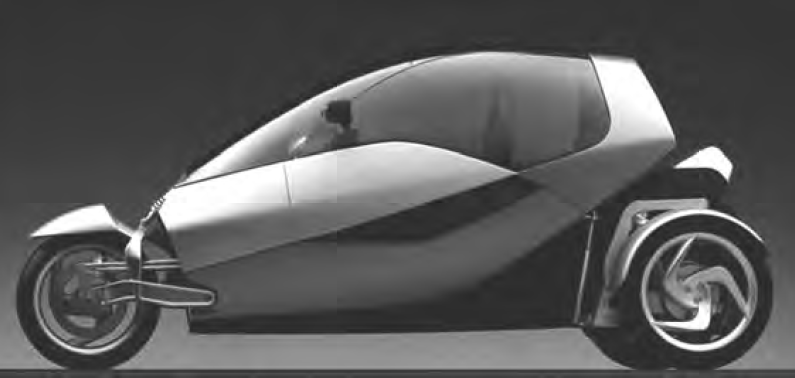
\includegraphics[width=.7\linewidth]{fig_01}
}%figues de la page de garde



\input{\repRel/Style/pagegarde_TD}

\setlength{\columnseprule}{.1pt}

\pagestyle{fancy}
\thispagestyle{plain}

\ifprof
\vspace{5.5cm}
\else
\vspace{4.9cm}
\fi

\def\columnseprulecolor{\color{bleuxp}}
\setlength{\columnseprule}{0.4pt} 

\setcounter{numques}{0}
%%%%%%%%%%%%%%%%%%%%%%%

\ifprof
%\begin{multicols}{2}
\else
\begin{multicols}{2}
\fi


\subsection*{Véhicule à trois roues Clever}
\begin{flushright}
\textit{Banque PT 2013 -- SIA.}
\end{flushright}
On s'intéresse au véhicule à 3 roues Clever.

\ifprof
\else
\begin{center}
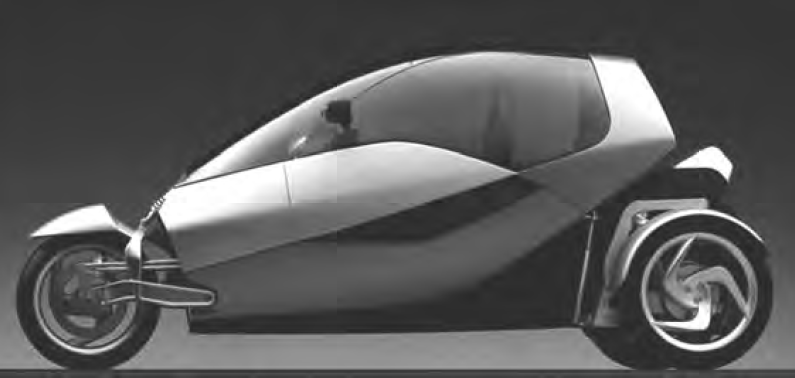
\includegraphics[width=.8\linewidth]{fig_01}
%\textit{}
\end{center}

 Le groupe motopropulseur est placé à l'arrière du véhicule. À l’avant, l’habitacle repose sur une roue de moto et pivote par rapport au bloc arrière autour d’une liaison pilotée angulairement par le biais de deux vérins hydrauliques. L'inclinaison est contrôlée par un ordinateur de bord en fonction de l'angle au volant et de la vitesse. 

\begin{center}
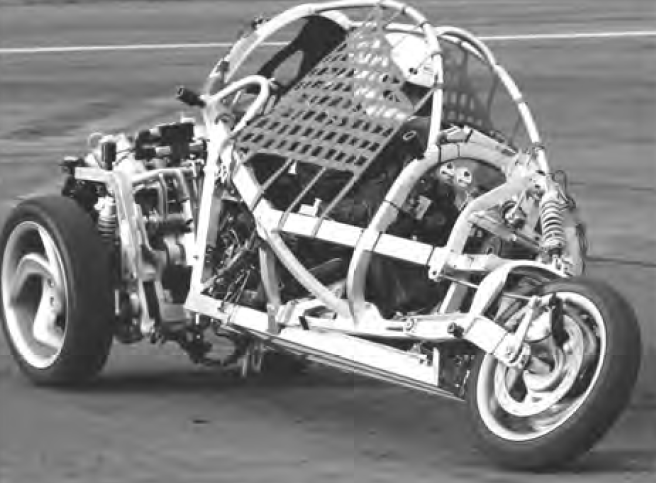
\includegraphics[width=.8\linewidth]{fig_02}
%\textit{}
\end{center}

Le système d’inclinaison de l’habitacle est assuré par un système constitué :
\begin{itemize}
\item d’un calculateur qui détermine le mouvement et la position à donner à l’habitacle en fonction des conditions
d’utilisation;
\item d’un système hydro-mécanique de transmission de puissance et d’adaptation de mouvement;
\item d’un système de contrôle de l’inclinaison de l’habitacle.
\end{itemize}

La chaîne de transmission de puissance et d’adaptation de mouvement est composée :
\begin{itemize}
\item d’une pompe à engrenages actionnée par le moteur à gaz via un système de poulies/courroie;
\item d’un circuit hydraulique;
\item de 2 vérins hydrauliques simple effet;
\item d’un système mécanique d’adaptation de mouvement afin de transformer le mouvement de translation des tiges des vérins en rotation de l’habitacle.
\end{itemize}


\begin{center}
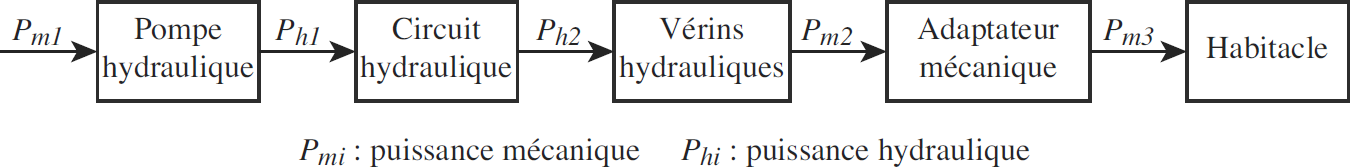
\includegraphics[width=\linewidth]{fig_03}
%\textit{}
\end{center}

\begin{center}
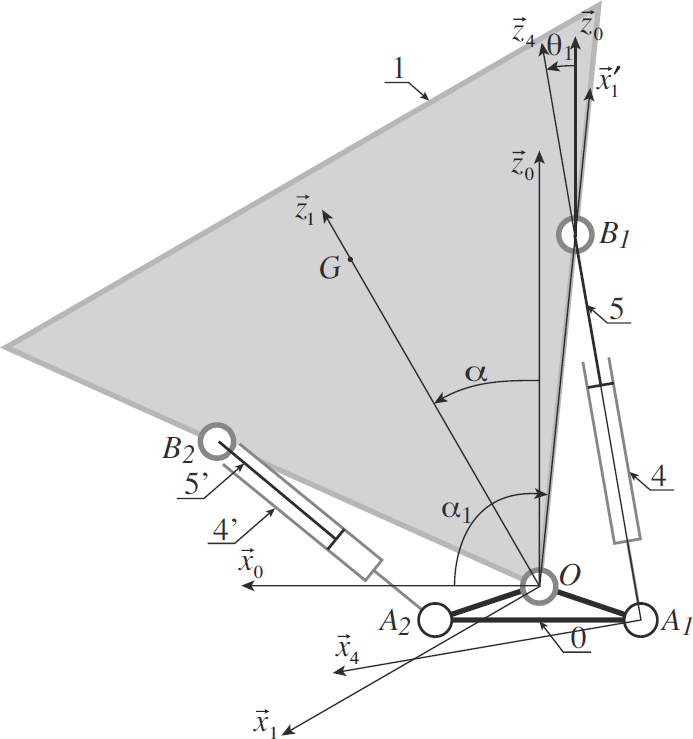
\includegraphics[width=.7\linewidth]{fig_04}
%\textit{}
\end{center}


Les deux vérins hydrauliques transforment la puissance hydraulique venant du servo-distributeur afin d’incliner l’habitacle. Ceux-ci sont disposées entre l’habitacle et le châssis du module arrière de propulsion. Le calculateur autorise ou non, l’alimentation en huile de l’un des vérins provoquant la sortie de tige, pendant que l’huile s'évacue de l’autre vérin. Ainsi l’habitacle s'incline du coté opposée au vérin alimenté. Lorsque l’habitacle est en position centrale, les tiges de vérins ont en position médiane.


Le circuit hydraulique est composé de 6 modules:
\begin{itemize}
\item une pompe à engrenages entraînée par le moteur à gaz;
\item un clapet anti-retour et une valve de décharge tarée pour s’enclencher à \SI{160}{bar} et se remettre en position fermée à \SI{100}{bar};
\item un accumulateur oléopneumatique de volume nominal \SI{1,4}{L};
\item un limiteur de pression;
\item un servo-distributeur à effet proportionnel 4/3 à centre fermé;
\item deux vérins simple effet, de diamètre \SI{32}{mm} pour chaque piston et de \SI{200}{mm} de course.
\end{itemize}

\fi

\question{Compléter le câblage du circuit hydraulique à partir du signe << * >>, ainsi que le schéma  du servo-distributeur.}

\ifprof
\begin{corrige}
\begin{center}
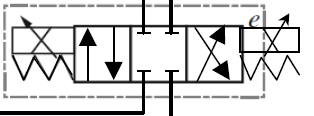
\includegraphics[width=.5\linewidth]{cor_01}
%\textit{}
\end{center}
\end{corrige}
\else\begin{center}
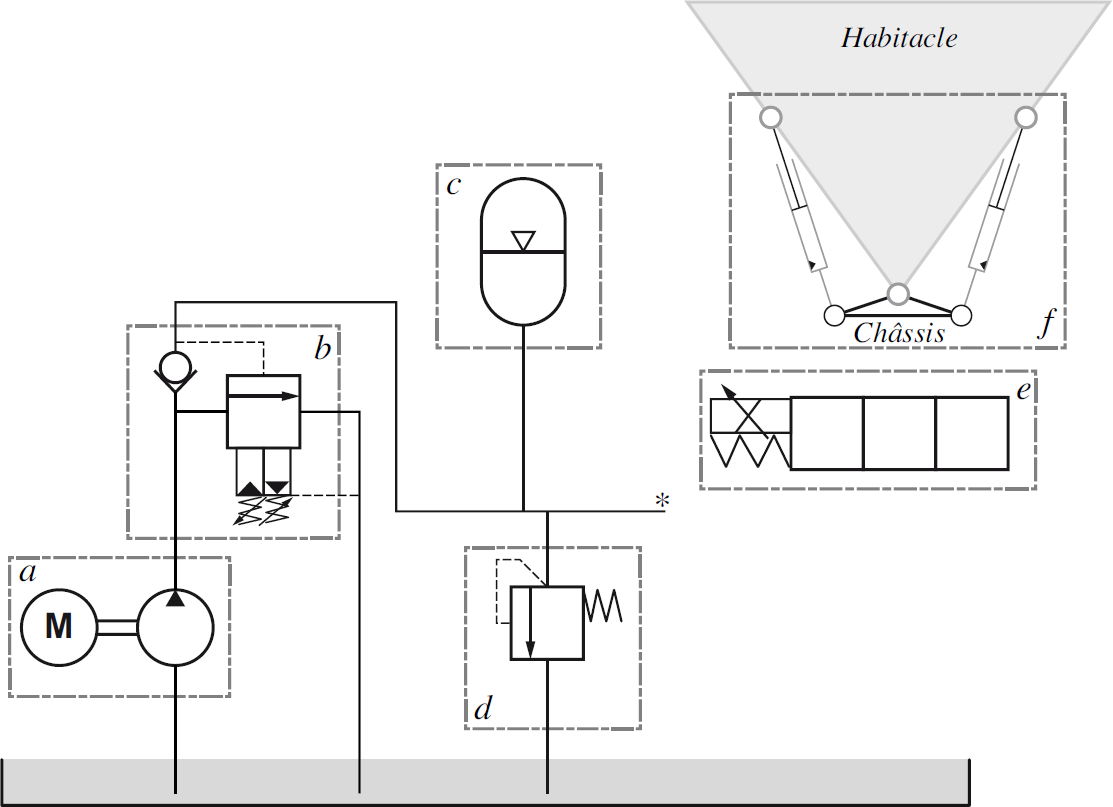
\includegraphics[width=\linewidth]{fig_05}
%\textit{}
\end{center}

\fi

Au démarrage du véhicule, la valve de décharge du module (b) est fermée. Le distributeur à effet proportionnel(e) est en position médiane, les vérins sont donc immobiles. La commande des vérins est initialement bloquée par une temporisation.

\question{En considérant les conditions initiales évoquées, expliquer, en commençant à l’instant de démarrage de la pompe, le comportement du circuit hydraulique en précisant clairement les différentes phases de fonctionnement. Quel est l’utilité de la temporisation ? On souhaite remplacer cette temporisation par un capteur. Préciser la grandeur qu’il devra mesurer. Donner un avantage et un inconvénient du remplacement de la temporisation par ce capteur.}
\ifprof
\begin{corrige}
Démarrage de la pompe et montée en pression du circuit avec remplissage de l’accumulateur (c).

À la fin de la temporisation le distributeur peut être commandé et ainsi alimenter les vérins.

Si la pression augmente trop, alors le limiteur de pression (d) renvoie une partie du fluide vers le
réservoir et si c’est insuffisant alors (b) permet une décharge du circuit (ouverture vers le réservoir
jusqu’à atteindre ne niveau bas réglé).

La temporisation permet d’attendre qu’un niveau de pression suffisant dans le circuit soit atteint.

Pour remplacer la temporisation on peut mesurer la pression dans le circuit ou plus simplement détecter
le niveau de pression satisfaisant pour le fonctionnement à l’aide d’un pressostat.

La solution utilisant un capteur de pression est plus sûre que la temporisation qui pourrait autoriser la
commande du distributeur alors que la pression dans le circuit est encore insuffisante.

(UPSTI). 
\end{corrige}
\else
\fi


\subsection*{Suspension pneumatique de véhicule de transport routier}
\setcounter{exo}{0}
\begin{flushright}
\textit{X--ENS PSI 2016.}
\end{flushright}

\ifprof
\else
La suspension assure la liaison élastique entre le châssis et les essieux. Elle permet principalement d’atténuer les accélérations verticales dues aux variations de profil de la chaussée, contribuant ainsi à l’amélioration du confort et à une meilleure tenue de route.

\begin{center}
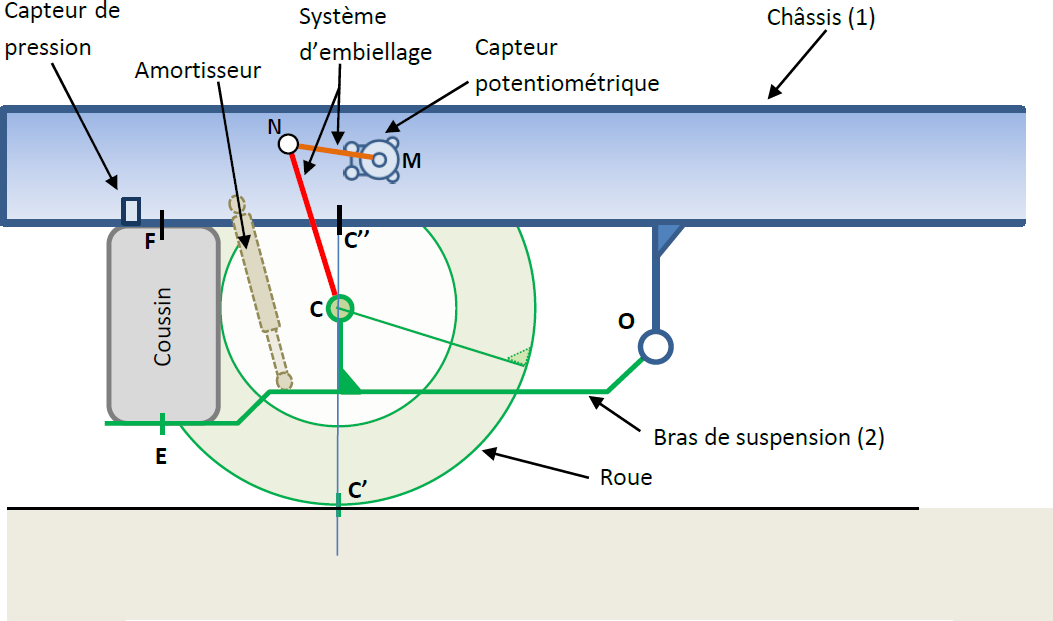
\includegraphics[width=\linewidth]{fig_06}
%\textit{}
\end{center}

Chaque roue possède une suspension pneumatique sur coussin pilotée par des électrovannes, en fonction de données mesurées par des capteurs de pression et des capteurs de position. Un calculateur envoie des commandes électriques aux électrovannes en fonction des besoins.

\begin{center}
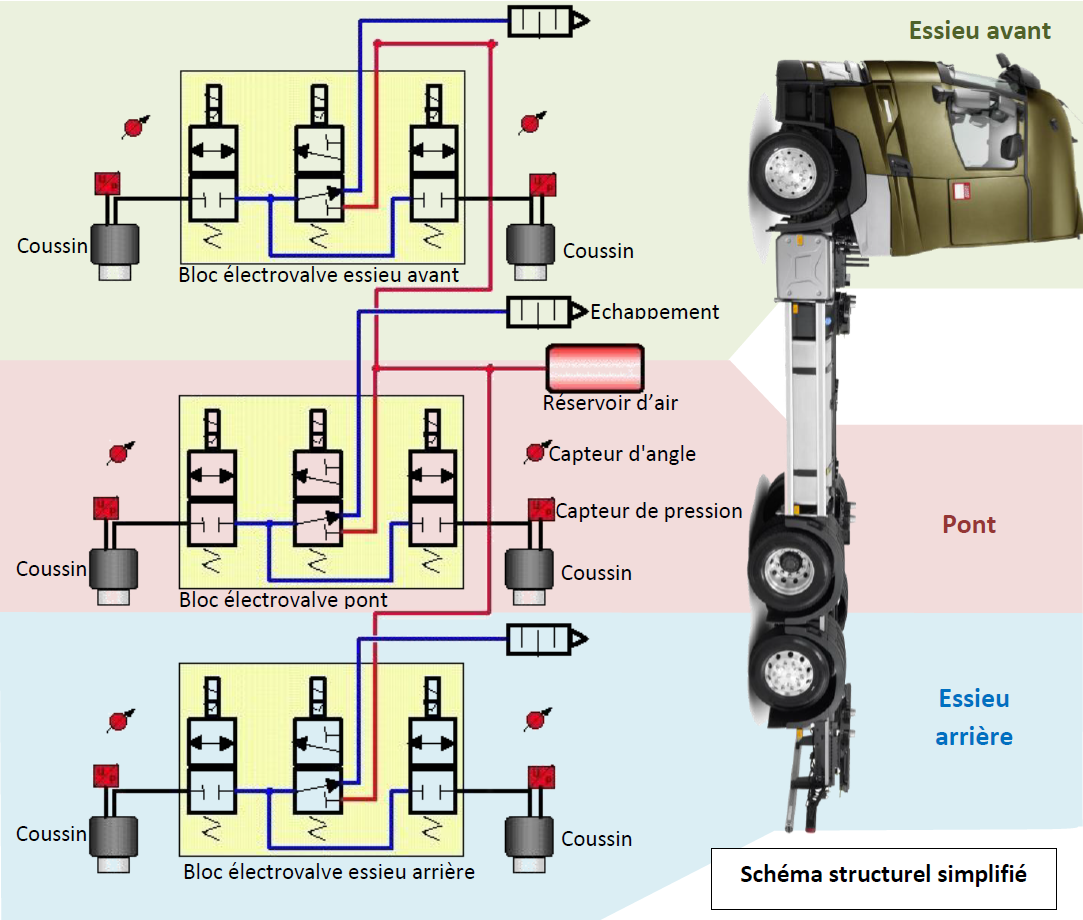
\includegraphics[width=\linewidth]{fig_07}
%\textit{}
\end{center}


\begin{center}
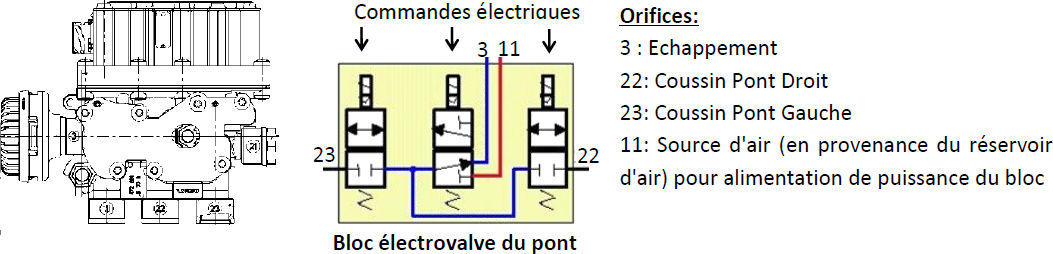
\includegraphics[width=\linewidth]{fig_08}
%\textit{}
\end{center}

Lorsque le niveau mesuré est inférieur à la valeur de consigne (niveau du châssis par rapport au sol), l’électrovalve est commandée de manière à provoquer le gonflage des coussins.
Lorsque le niveau a dépassé la consigne, on commande la vidange des coussins.

\fi
\question{Représenter les trois distributeurs dans la situation de gonflage, puis dans la situation de vidange des coussins.
}
\ifprof
\begin{corrige}
\begin{center}
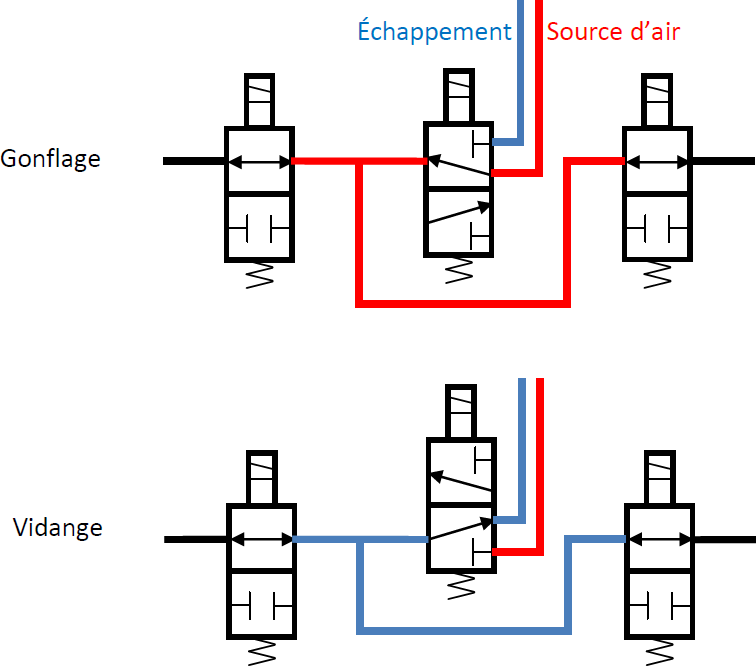
\includegraphics[width=.5\linewidth]{cor_02}
%\textit{}
\end{center}
\end{corrige}
\else
\fi


\subsection*{Bouée houlomotrice}
\setcounter{exo}{0}
\begin{flushright}
\textit{CCP PSI 2016.}
\end{flushright}


\ifprof
\else
L’énergie produite à partir de la houle est appelée houlomotrice (ou énergie des vagues). Cette énergie est le plus souvent
transformée en énergie électrique.

\begin{center}
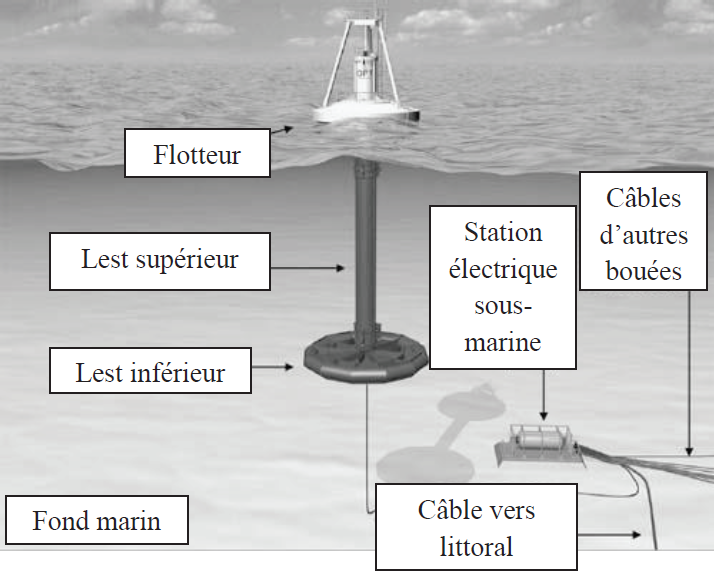
\includegraphics[width=\linewidth]{fig_09}
%\textit{}
\end{center}

Le système de conversion d'énergie est schématisé sur la figue suivante.

Le vérin hydraulique est entraîné par le mouvement relatif de translation entre le flotteur et le lest.
La translation du piston par rapport au cylindre du vérin est donc également paramétrée par le
déplacement $z(t)$ par rapport à la position d’équilibre. La section utile du piston est notée $S_p$. Les
pressions dans les chambres supérieure et inférieure du vérin sont notées respectivement $P_1$ et $P_2$.

Un réservoir accumulateur haute pression (a) et un réservoir accumulateur basse pression (b)
permettent de maintenir les pressions $P_a$ (pression d'admission du moteur hydraulique) et $P_b$
(pression de refoulement du moteur hydraulique) quasi-constantes en régime établi.

Un ensemble de clapets anti-retour permet de générer un débit volumique unidirectionnel $Q_m(t)$
vers le moteur hydraulique, quel que soit le sens de déplacement du piston. Les pertes induites par
ce circuit redresseur seront négligées. On pourra alors considérer en régime établi, et en première
approximation, les relations suivantes entre les pressions dans les réservoirs et dans les chambres du
vérin : $P_a = \text{max} \left(P_1,P_2\right)$ et $P_b = \text{min} \left(P_1,P_2\right)$.

\fi


\question{Compléter les zones en pointillés du schéma hydraulique en dessinant
les clapets anti-retour conformément à la description précédente.}
\ifprof
\begin{corrige}
\begin{center}
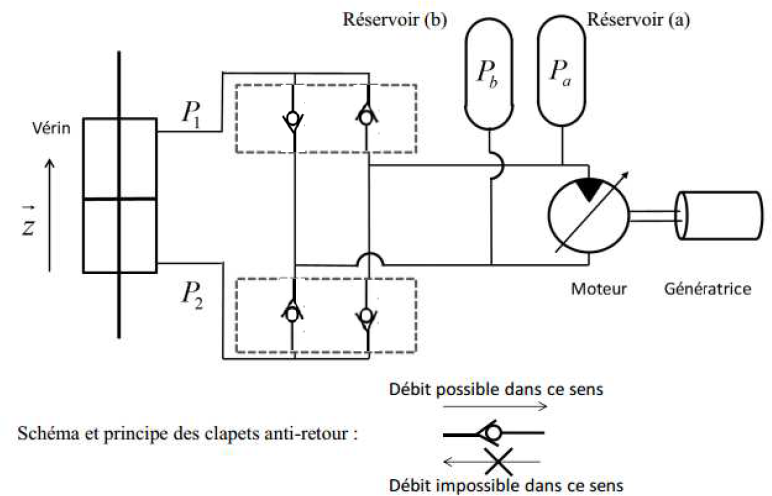
\includegraphics[width=.5\linewidth]{cor_03}
%\textit{}
\end{center}
\end{corrige}
\else


\begin{center}
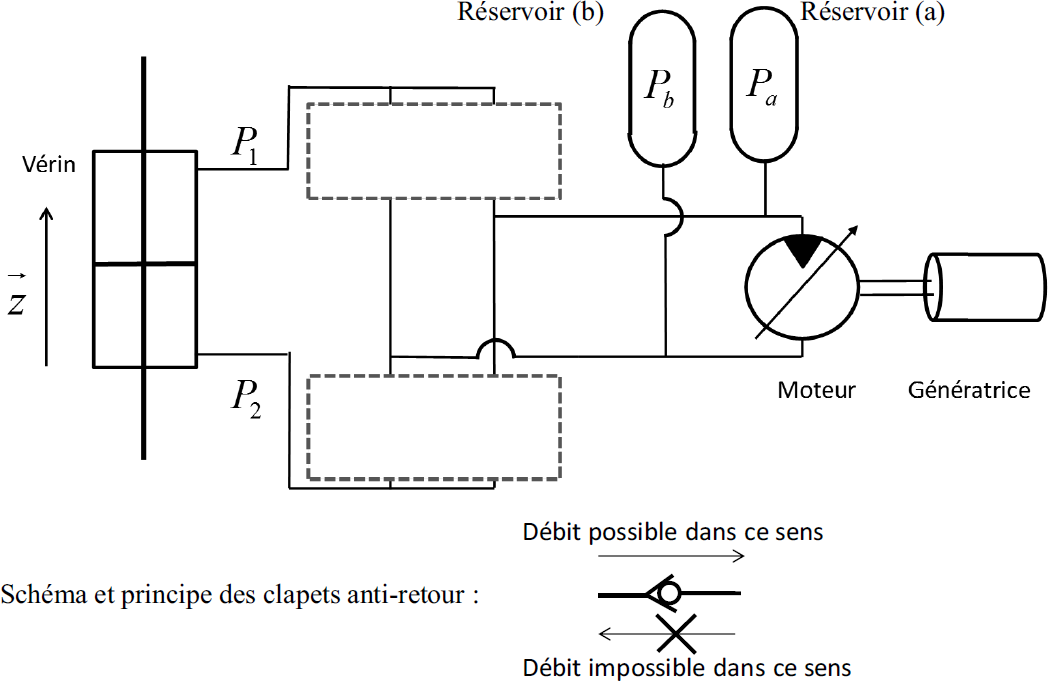
\includegraphics[width=\linewidth]{fig_10}
%\textit{}
\end{center}
\fi
\ifprof
\else
\end{multicols}

\fi
